\documentclass[11pt]{article}

\pagestyle{empty}                         %%%% No page Numbering
 
% Mathews packages....
\usepackage{amsbsy,amsmath,amssymb,psfig} 
\usepackage{times,mathpi,mathptm} 
\usepackage{graphicx,psfrag,rotating,subfigure} 

\begin{document}	
\section{Calculation of the sparsity pattern for Mixed formulation}
	
In the mesh migration problem, it is useful to use a first order
element-element adjancy matrix when a mixed formulation is being used
by the solver. To see why, consider
Figure~\ref{fig:mixedgraph}. Normally the yellow elements define the
mesh overlap, or halo, between two domains. In the case of a mixed
formulation, some field values are stored and solved on a more sparce
matrix pattern. For the mixed formulation considered here, all
elements adjacent to yellow elements, are also required on the
neighbouring domain. The elements of interest are coloured blue in
Figure~\ref{mixedgrapg}. 

Define $\pmb{E}$ as the element-element adjancy matrix over all the
domains where
\begin{displaymath}
E_{ij} = \left\{ \begin{array}{ll}
1 & \textrm{if element $i$ shares nodes with element $j$ and $i \ne j$,}\\
0 & \textrm{otherwise}
\end{array} \right.
\end{displaymath}

\begin{figure}[h]\label{fig:mixedgraph}
\centering
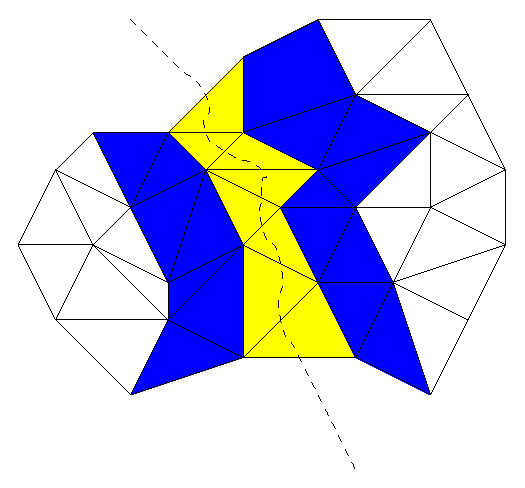
\includegraphics[width=80mm]{images/mixed}
\caption{Yellow indicates elements in the halo between two domains
divided by the dashed line. The blue elements indicates the additional
elements that need to be communicated to the neighbouring domains in
the mixed formulation}
\end{figure} 

Next we define $\pmb{D}_s$ is the element distribution across the domains
\begin{displaymath}
D_{s_i} = \left\{ \begin{array}{ll}
1 & \textrm{if element $i$ has nodes assigned to domain $s$,}\\
0 & \textrm{otherwise}
\end{array} \right.
\end{displaymath}
Thus, the yellow halo elements between domains $s$ and $r$ can be
defined by $pmb{H}_{sr} = \pmb{D}_s \otimes \pmb{D}_r$. 

Finally, let us define $\pmb{B}_{sr}$ as the non-halo elements in
domain $s$, which have to be sent with some specific field values to
domain $r$;
\begin{equation}
B_{sr_i} = S( (H_{sr_i}\pmb{E}_i ).D_s )
\end{equation}

where the function $S$ is defined by
\begin{displaymath}
S(x) = \left\{ \begin{array}{ll}
1 & \textrm{for $x \ne 0$,}\\
0 & \textrm{otherwise}
\end{array} \right.
\end{displaymath}

\end{document} 








